\documentclass[10pt,a4paper]{article}
\usepackage[utf8]{inputenc}
\usepackage[francais]{babel}
\usepackage{color}
\usepackage[T1]{fontenc}
\usepackage{amsmath}
\usepackage{amsfonts}
\usepackage{amssymb}
\usepackage{graphicx}
\author{Guillaume Huysmans et Florent Delgrange}
\title{Intelligence Artificielle\\Pré-projet}
\begin{document}
\maketitle
\section{Introduction}
Il nous a été demander d'implémenter 3 IA pour le jeu de Nim.
\begin{enumerate}
\item Une IA aléatoire qui gagne en un tour si elle en a la possibilité et joue aléatoirement sinon.
\item Une IA qui joue optimalement à chaque tour "si elle en a la possibilité" (nous reviendrons sur cette notion plus tard) et aléatoirement sinon.
\item Une IA coopérative qui permet de jouer à deux contre un.
\end{enumerate}
Nous allons, au cours de ce rapport, expliquer les algorithmes que nous avons employés pour résoudre ces problèmes.

\section{IA aléatoire améliorée}
L'IA joue aléatoirement jusque quand il est possible pour elle de faire un coup gagnant. Un coup gagnant correspond au moment dans le jeu où il reste, au plus, autant de pions que le nombre de pions qu'on a le droit de déplacer.\\
Soient m, le nombre de pions restant et n le nombre de pions maximum qu'on est autorisé de déplacer. Nous nous trouvons dans une telle situation ssi
\[m\mod n = n\]
Notre IA joue aléatoirement jusqu'à atteindre cette propriété. Si elle l'atteint, alors elle retire n pions et gagne.

\section{IA Gagnante}
Soient m, le nombre de pions restants et n le nombre de pions maximum qu'on est autorisé de déplacer. Un coup est dit "optimal" si à chaque tour, celui-ci correspond à \[coup \ optimal\ = m \mod (n+1)\ ssi\ m \mod (n+1) \neq 0 \]
Dans le cas contraire, l'IA ne sait pas jouer optimalement et joue aléatoirement.\\
Afin d'illustrer cette propriété, nous allons nous baser sur un graphe que nous avons généré.
\begin{figure}
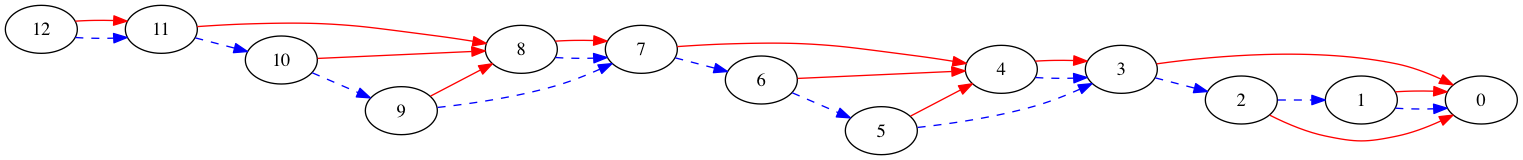
\includegraphics[scale=0.2]{nim.png}
\label{nim12}
\caption{Déroulement d'un jeu de Nim}
\end{figure}
La figure ~\ref{nim12} représente l'évolution d'un jeu de Nim tel que m=12 et n=3. Nous considérons pour cet exemple, par souci de lisibilité, que quand l'IA ne peut pas faire un coup gagnant, il ne retire qu'un pion à la place de jouer aléatoirement. Le parcours correspondant à cette IA est décrit par le chemin décrit en {\color{red} rouge}. Les sommets de ce graphe représentent le nombre de pions restants et les arcs, le nombre de pions que l'IA retire. \\
L'IA gagnante va donc "bloquer" l'adversaire à chaque tour, l'empêchant d'arriver au cas  où m mod (m+1) = n (le cas où il reste au plus autant de jetons que de jetons maximum qu'il est possible de retirer). Lorsque l'IA gagnante tombe dans ce cas de base, il gagne (et il y arrivera obligatoirement en premier dans le cas d'un jeu de Nim à 2 joueurs).

\section{IA Coopérative}
Deux joueurs ligués doivent être surs de gagner c'est à dire que le joueur 1 ou le joueur 2 doit gagner la partie.
Cette IA a pour but de permettre au joueur qui joue au tour suivant de toujours avoir la possibilité de faire un coup optimal.
Soient m, le nombre de pions restants et n le nombre de pions maximum qu'on est autorisé de déplacer. L'IA permet au joueur suivant de faire un coup optimal (comme défini à la section précédente) si et seulement si l'IA retire x jetons, x étant défini de la façon suivante :
\[ \begin{cases}
	\text{(1) } x \in [1, min(n, m)] \text{ (aléatoirement)} \ & \quad \text{si } m \mod (n+1) = 0 \ ou \ m \mod (n+1) = n\\
	\text{(2) } x = 2 & \quad \text{si } (m-1) \mod (n+1) = 0 \\
	\text{(3) } x = 1 &\ \quad \text{sinon }\\
	\end{cases}
\]
Pour illustrer cette propriété, nous nous référons de nouveau à la figure ~\ref{nim12}. Le parcours correspondant à cette IA est décrit par le chemin décrit en {\color{blue} bleu}. \\
Dans le cas (1), par le fait que m mod n+1 = 0, n'importe quel coup porté par le joueur jouant au tour suivant aura la possibilité d'être optimal. De plus, si m (mod n+1) = n, alors on peut également jouer aléatoirement car cela signifie qu'il reste au plus n pions et donc que l'IA coopérative permet soit au joueur suivant de gagner, soit gagne en retirant le nombre de pions restants.\\
Le cas (2) correspond au cas où, si l'IA retire 1 jeton, celle-ci bloque le joueur suivant et lui interdit de jouer optimalement. L'IA retire alors 2 jetons pour assurer au joueur suivant la possibilité de placer un coup optimal.\\
Finalement, le cas (3) ne nous permet pas de jouer aléatoirement dans [1, n] car on pourrait encore une fois bloquer le joueur suivant. Cependant, il est tout à fait possible de retirer 1 jeton pour être sur que le joueur suivant soit sûr de jouer optimalement. \\
Il est donc trivial que associée à l'IA gagnante, les deux joueurs ligués seront certains de gagner dans des parties de 3 joueurs avec n $\geq$ 2.  En effet, l'IA coopérative permettra, à chaque tour, à l'IA gagnante de bloquer l'adversaire.

\section{Remarque}
Nous n'aurions voulu créer qu'une seule IA capable de décider d'aider le joueur suivant si il est dans son équipe ou d'attaquer celui-ci dans le cas où le joueur suivant est un adversaire, mais le framework ne permet malheureusement pas à un joueur de déterminer qui joue avec lui.

\end{document}